\section{Theoretical Analysis and Simulation Results}
\label{sec:analysis}

In this section, the circuit shown in Figure \ref{fig:lab2} is analysed
theoretically and is simulated too, following the order of the topics that are in presentation of this laboratory. %melhorar isto
\subsection{Topic 1 - T/S}
This topic corresponds to the first theoretical and the first simulation topics.
\par
Using the nodal method (based on the Kirchhoff's Current Law (KCL)), since we have 8 different nodes we must have 8 different 
equations in order to have a solvable system of equations, therefore we obtain the following set of equations:

\begin{equation} 	%NODE 0
  V_0=0          ;
  \label{eq:1}
\end{equation}

\begin{equation} 	%NODE 1
  V_1=V_S           ;
  \label{eq:2}
\end{equation}

\begin{equation} 	%NODE 2 
  \frac{V_2-V_1}{R_1}+\frac{V_2-V_5}{R_3}+\frac{V_2-V_3}{R_2}=0    ;
  \label{eq:3}
\end{equation}

\begin{equation} 	%NODE 3
  \frac{V_3-V_2}{R_2}-K_b\times(V_2-V_5)=0    ;
  \label{eq:4}
\end{equation}

\begin{equation} 	%NODE 5
  \frac{V_5-V_0}{R_4}+\frac{V_5-V_2}{R_3}+\frac{V_5-V_6}{R_5}+\frac{V_8-V_7}{R_7}-I_C=0 \iff \frac{V_3-V_0}{R_4}+\frac{V_5-V_2}{R_3}+\frac{V_5-V_6}{R_5}+\frac{V_8-V_7}{R_7}=0    ;
  \label{eq:5}
\end{equation}

\begin{equation} 	%NODE 6
  \frac{V_6-V_5}{R_5}+K_b\times(V_2-V_5)+I_C=0 \iff \frac{V_6-V_5}{R_5}+K_b\times(V_2-V_5)=0   ;
  \label{eq:6}
\end{equation}

\begin{equation} 	%NODE 7
  \frac{V_7-V_0}{R_6}+\frac{V_7-V_8}{R_7}=0 \iff \frac{V_7}{R_6}+\frac{V_7-V_8}{R_7}=0   ;
  \label{eq:7}
\end{equation}

\begin{equation} 	%NODE 8
  V_5-V_8=K_d\times\frac{V_7}{R_6}   ;
  \label{eq:8}
\end{equation}

being Equation 1 referent to node 0, Equation 2 to node 1, Equation 3 to node 2, Equation 4 to node 3, Equation 5 to node 5, Equation 6 to node 6, Equation 7 to node 7
and Equation 8 to node 8.  
In equations 5 and 6, considering $I_c = C*\frac{dVc}{dt}$ and being the circuit static, $V_c$ is a constant so $I_c$ is zero.
%Using Octave, we can easily solve this system of equations using matrix operations resulting in following results:

The results of the simulation and the theoretical results are presented in the following tables:

\begin{table}[h]
  \centering
  \begin{tabular}{|l|r|}
    \hline    
    {\bf Name} & {\bf Value [A or V]} \\ \hline
    V0 & 0.00000000000\\ \hline 
V1 & 5.19519931250\\ \hline 
V2 & 4.98987457574\\ \hline 
V3 & 4.55661925037\\ \hline 
V5 & 5.01921537838\\ \hline 
V6 & 5.65928593115\\ \hline 
V7 & -2.01261748847\\ \hline 
V8 & -3.01962752440\\ \hline 

  \end{tabular}
  \caption{Theoretical Results for topic 1}
  \label{tab:tabela1}
\end{table}

 \begin{table}[h]
  \centering
  \begin{tabular}{|l|r|}
    \hline    
    {\bf Name} & {\bf Value [A or V]} \\ \hline
    @c1[i] & 0.000000e+00\\ \hline
@gb[i] & -2.08664e-04\\ \hline
@r1[i] & 1.992363e-04\\ \hline
@r2[i] & 2.086637e-04\\ \hline
@r3[i] & -9.42740e-06\\ \hline
@r4[i] & 1.200363e-03\\ \hline
@r5[i] & -2.08664e-04\\ \hline
@r6[i] & 1.001127e-03\\ \hline
@r7[i] & 1.001127e-03\\ \hline
v(1) & 5.195199e+00\\ \hline
v(2) & 4.989875e+00\\ \hline
v(3) & 4.556619e+00\\ \hline
v(5) & 5.019215e+00\\ \hline
v(6) & 5.659286e+00\\ \hline
v(7) & -2.01262e+00\\ \hline
v(8) & -2.01262e+00\\ \hline
v(9) & -3.01963e+00\\ \hline
                                   
  \end{tabular}
  \caption{Simulation Results for topic 1}
  \label{tab:tabela2}
\end{table}

As we can see both tables have the same results and the reason for that is that ngspice uses the same models (KCL/KVL) as we used in octave.
%----------------------------------------------------------------------------------------------------------------------
%----------------------------------------------------------------------------------------------------------------------
\subsection{Topic 2-T/S}
This topic corresponds to the second theoretical and the second simulation topics.
Using the nodal method (based on the Kirchhoff's Current Law (KCL)), since we have 8 different nodes we must have 8 different 
equations in order to have a solvable system of equations, therefore we obtain the following set of equations:
\begin{equation} 
  V_0=0          ;
  \label{eq:1.1}
\end{equation}

\begin{equation} 
  V_1=0          ;
  \label{eq:2.1}
\end{equation}

\begin{equation} 
  \frac{V_2-V_1}{R_1}+\frac{V_2-V_5}{R_2}=0          ;
  \label{eq:3.1}
\end{equation}

\begin{equation} 
  \frac{V_3-V_2}{R_2}-K_b\times(V_2-V_5)=0          ;
  \label{eq:4.1}
\end{equation}

\begin{equation} 
  \frac{V_7}{R_6}+\frac{V_7-V_8}{R_7}=0          ;
  \label{eq:6.1}
\end{equation}

\begin{equation} 
  V_6-V_8=V_x         ;
  \label{eq:7.1}
\end{equation}

\begin{equation} 
  V_5-V_8+K_d\times\frac{V_7}{R_6}=0          ;
  \label{eq:8.1}
\end{equation}

\begin{equation} 
  \frac{V_5}{R_4}+\frac{V_5-V_2}{R_3}+\frac{V_5-V_6}{R_5}+\frac{V_8-V_7}{R_7}+\frac{V_6-V_5}{R_5}+K_b(V_2-V_5)=0 \iff \frac{V_5}{R_4}+\frac{V_5-V_2}{R_3}+\frac{V_8-V_7}{R_7}+K_b(V_2-V_5)=0        ;
  \label{eq:8.2}
\end{equation}

The results of the simulation and the theoretical results are presented in the following tables:

\begin{table}[h]
  \centering
  \begin{tabular}{|l|r|}
    \hline    
    {\bf Name} & {\bf Value [A or V]} \\ \hline
    Ic & -0.00282933503\\ \hline 
Req & -3067.47464193000\\ \hline 
Tau & 0.00319445744\\ \hline 
V0 & 0.00000000000\\ \hline 
V1 & 0.00000000000\\ \hline 
V2 & -0.00000000000\\ \hline 
V3 & 0.00000000000\\ \hline 
V5 & 0.00000000000\\ \hline 
V6 & 8.67891345555\\ \hline 
V7 & -0.00000000000\\ \hline 
V8 & -0.00000000000\\ \hline 

  \end{tabular}
  \caption{Theoretical Results for topic 2}
  \label{tab:tabela3}
\end{table}

\begin{table}[h]
  \centering
  \begin{tabular}{|l|r|}
    \hline    
    {\bf Name} & {\bf Value [A or V]} \\ \hline
    @gb[i] & 1.053111e-17\\ \hline
@r1[i] & -1.00553e-17\\ \hline
@r2[i] & -1.05311e-17\\ \hline
@r3[i] & 4.757942e-19\\ \hline
@r4[i] & 2.124111e-18\\ \hline
@r5[i] & -2.82934e-03\\ \hline
@r6[i] & 1.734723e-18\\ \hline
@r7[i] & 1.830908e-18\\ \hline
v(1) & 0.000000e+00\\ \hline
v(2) & 1.036259e-14\\ \hline
v(3) & 3.222868e-14\\ \hline
v(5) & 8.881784e-15\\ \hline
v(6) & 8.678914e+00\\ \hline
v(7) & -3.48740e-15\\ \hline
v(8) & -3.48740e-15\\ \hline
v(9) & -5.32907e-15\\ \hline
					
  \end{tabular}
  \caption{Simulation Results for topic 2}
  \label{tab:tabela4}
\end{table}

As we can see both tables have the same results and the reason for that is that ngspice uses the same models (KCL/KVL) as we used in octave.
This procedure is important to allow us to compute the equivalent resistor in the circuit which will be used in the calculation of the natural solution.
In ngspice, this allows us to present the natural solution in node 6 as will be presented in the next topic. 

\newpage
%----------------------------------------------------------------------------------------------------------------------
%----------------------------------------------------------------------------------------------------------------------
\subsection{Topic 3-T/S}
This topic corresponds to the third theoretical and the third simulation topics.

\begin{figure}[h!]
            \centering
            \subfigure[]{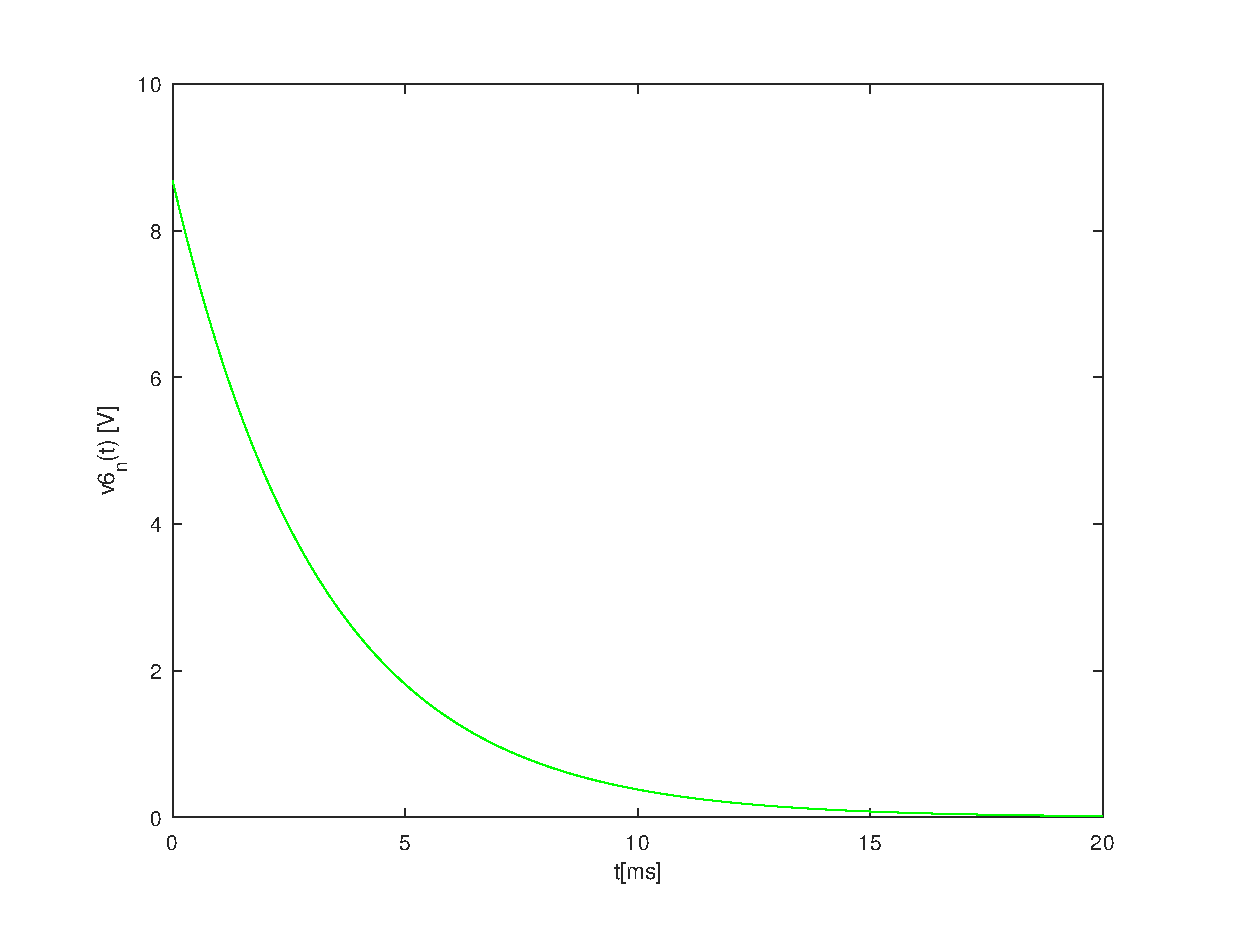
\includegraphics[width=0.49\textwidth]{v6_n.eps}} 
            \subfigure[]{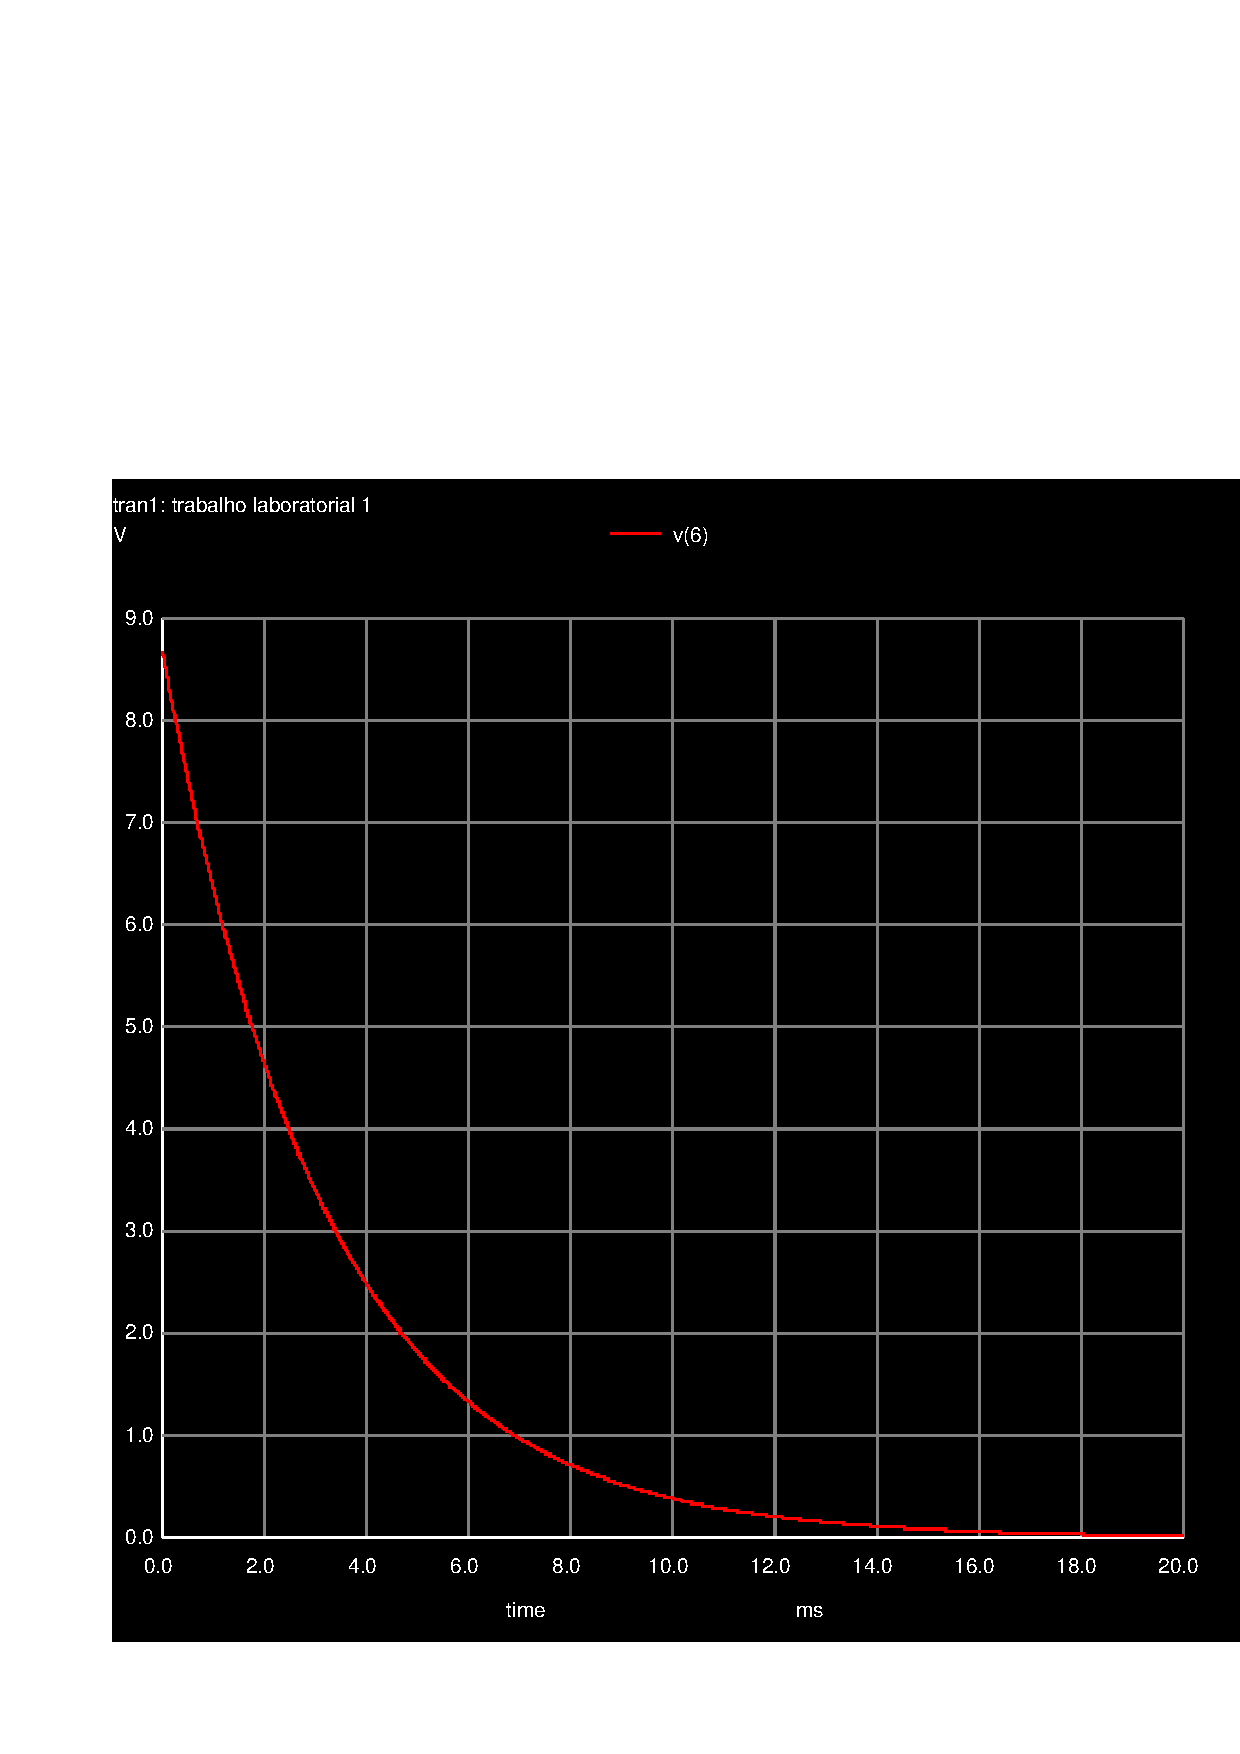
\includegraphics[width=0.40\textwidth]{trans.pdf}} 
            \caption{(a) Natural solution of V6 using octave (b) Natural solution of V6 using ngspice }
            \label{fig:icte}
\end{figure}

Looking to the graphics, we can see that both produce similar results. 
%and the little diferences exist because the use a different number of points to make a plot.
%----------------------------------------------------------------------------------------------------------------------
%----------------------------------------------------------------------------------------------------------------------
\newpage
\subsection{Topic 4-T}
This topic corresponds to the fourth theoretical.


\begin{table}[h]
  \centering
  \begin{tabular}{|l|r|}
    \hline    
    {\bf Name} & {\bf Value [A or V]} \\ \hline
    V0 & 0.00000000000+(0.00000000000)j\\ \hline 
V1 & 0.00000000000+(-1.00000000000)j\\ \hline 
V2 & -0.00000000000+(-0.96047798662)j\\ \hline 
V3 & -0.00000000000+(-0.87708266349)j\\ \hline 
V5 & -0.00000000000+(-0.96612566265)j\\ \hline 
V6 & -0.08302511326+(0.57709770658)j\\ \hline 
V7 & 0.00000000000+(0.38739947544)j\\ \hline 
V8 & 0.00000000000+(0.58123420157)j\\ \hline 

  \end{tabular}
  \caption{Theoretical results of topic 4}
  \label{tab:tabela5}
\end{table}

%---------------------------
\begin{figure}[ht] \centering
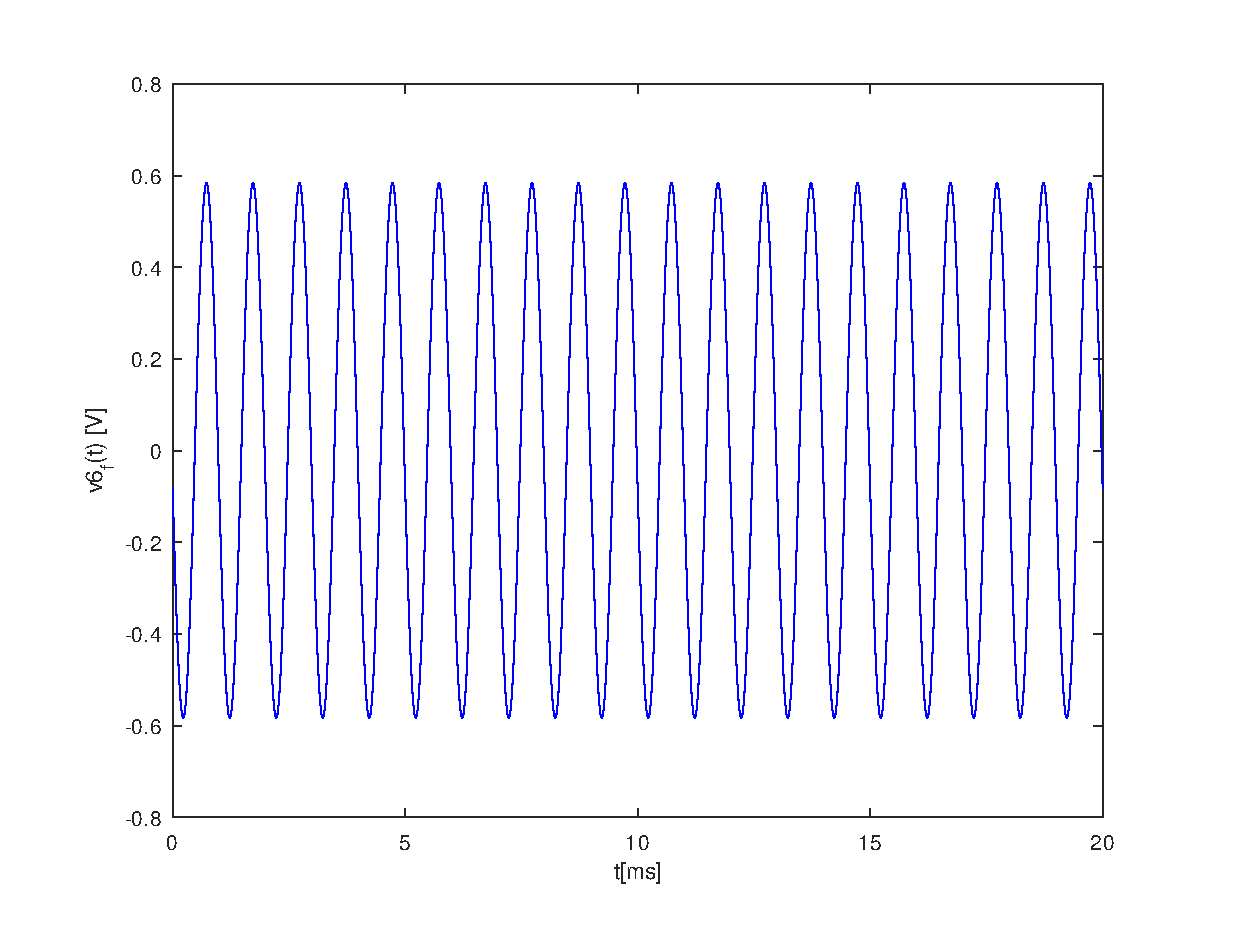
\includegraphics[width=0.5\linewidth]{v6_f.eps}
\caption{Forced solution of V6}
\label{fig:v6_f}
\end{figure}

Using phasors and apllying the nodal method, we obtained the phasors of all nodes, in particular the node 6 phasor which when multiplied
by $exp(jwt)$ corresponds to the forced solution. The aspect of the graph is like we expected, a sinuosoidal wave. 
%----------------------------------------------------------------------------------------------------------------------
%----------------------------------------------------------------------------------------------------------------------
\newpage
\subsection {Topic 5-T/S} 
This topic corresponds to the fifth theoretical and the fourth simulation topics.

\begin{figure}[h!]
            \centering
            \subfigure[]{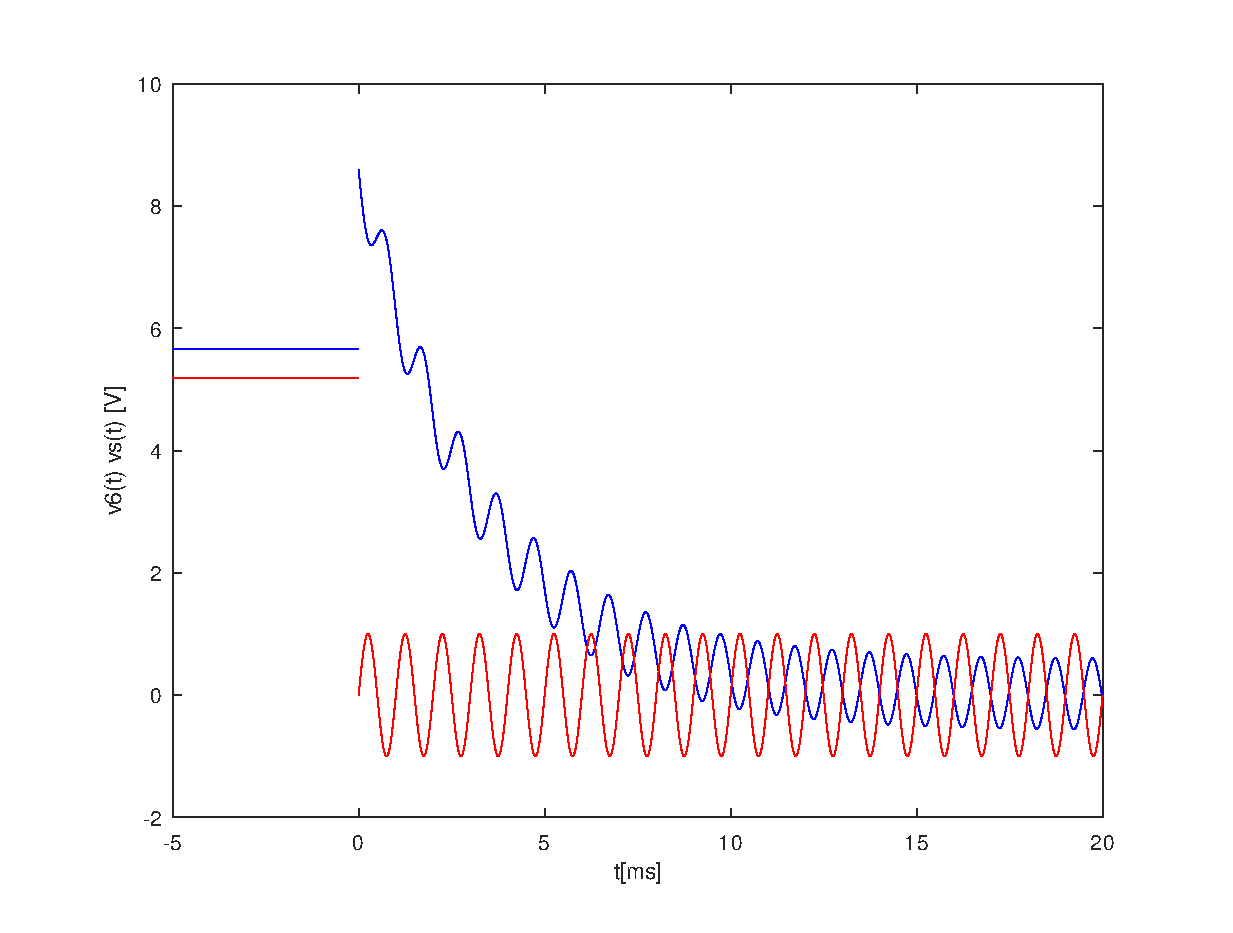
\includegraphics[width=0.49\textwidth]{v6_vs.eps}} 
            \subfigure[]{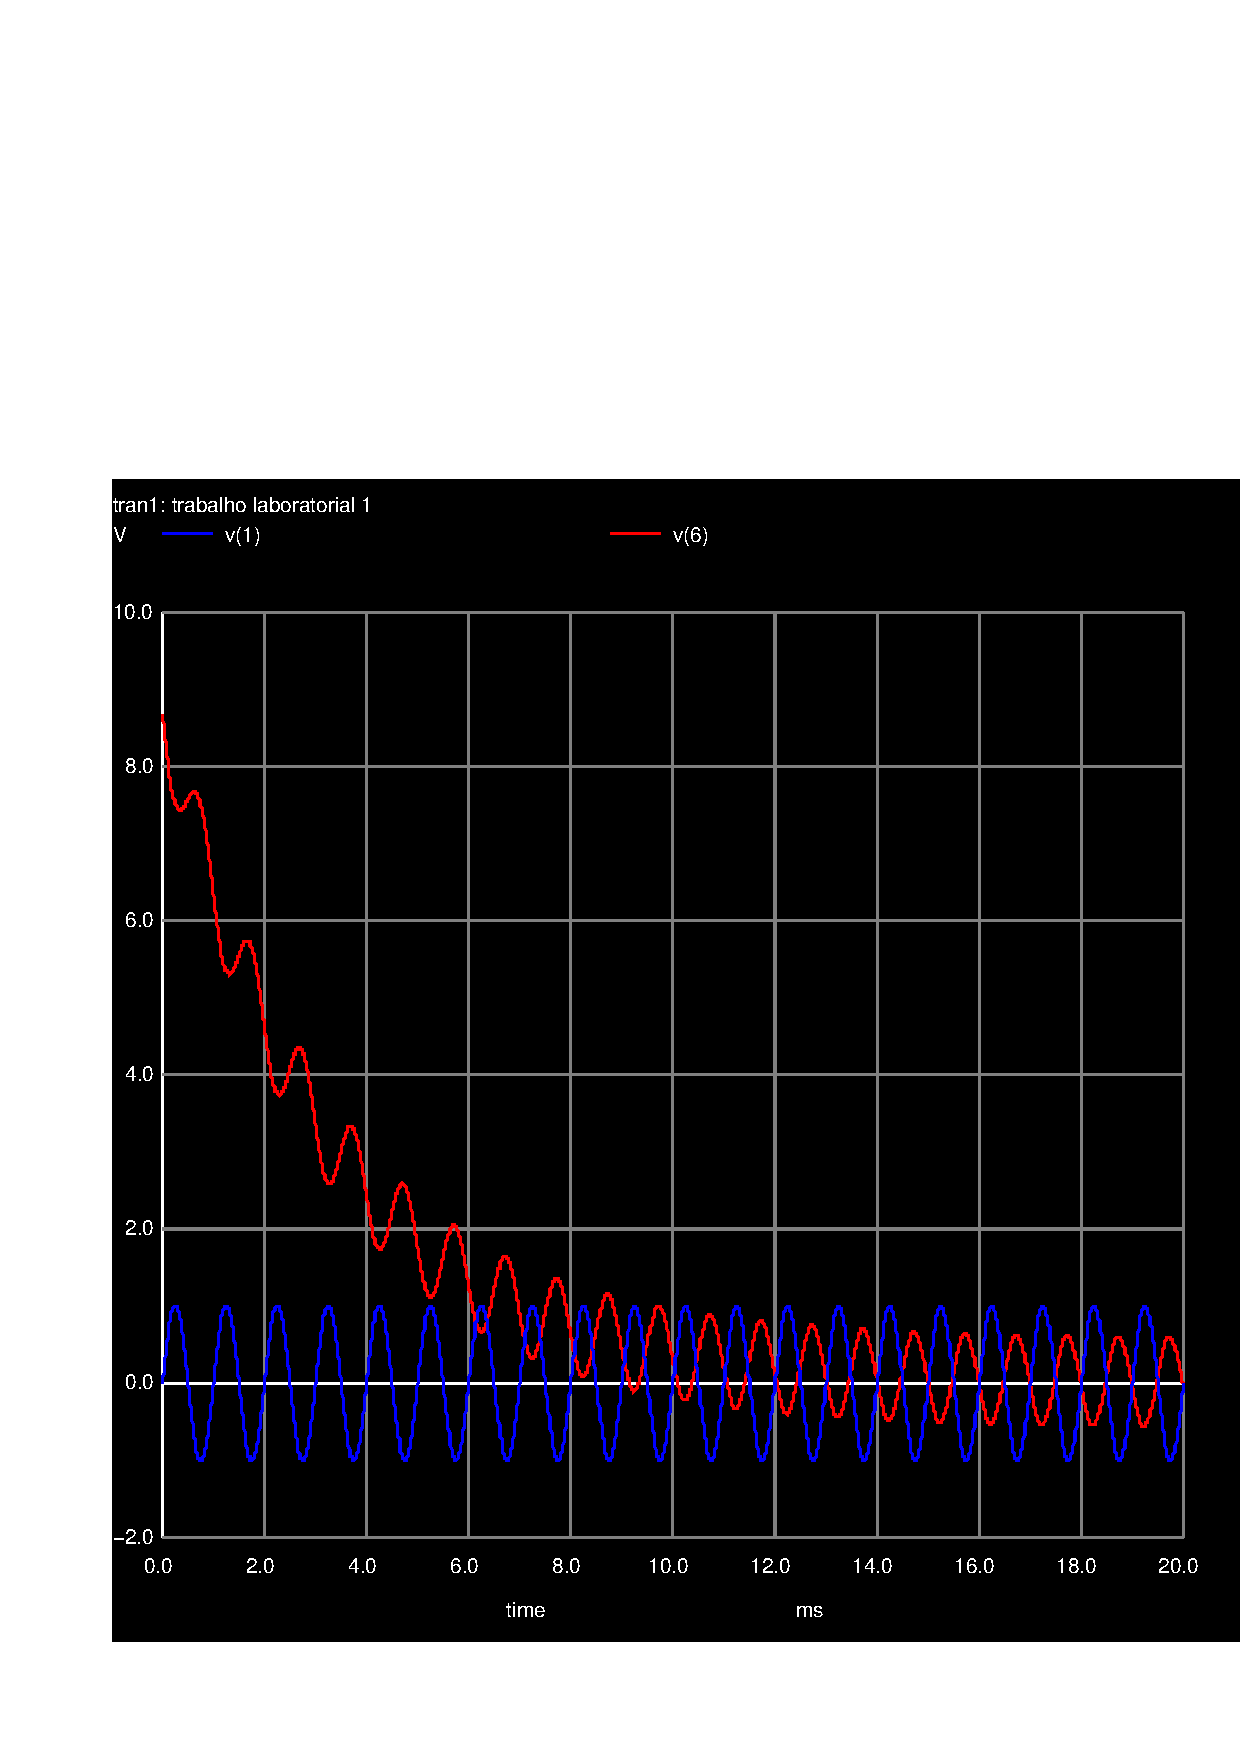
\includegraphics[width=0.40\textwidth]{trans2.pdf}} 
            \caption{(a) Solution to V6 and Vs using octave (b) Solution to V6 and Vs using ngspice}
            \label{fig:icer}
\end{figure}

In octave, to obtain the solution for V6 we just add the natural and forced solution. In ngspice, we did a transient analysis to obtain V6 solution.
As we can see, both figures look the same for V6 and obviously for Vs.



%----------------------------------------------------------------------------------------------------------------------
%----------------------------------------------------------------------------------------------------------------------

\subsection {Topic 6-T/S}
This topic corresponds to the sixth theoretical and the fifth simulation topics.

For the frequency analysis, in octave we chose to solve the nodal method with frequency as a symbolic variable. 
This procedure takes a few more seconds but ensures that we obtain the results without any approximation.
Another advantage of this method is that we obtain all nodes frequency dependence.

\begin{figure}[h!]
            \centering
            \subfigure[]{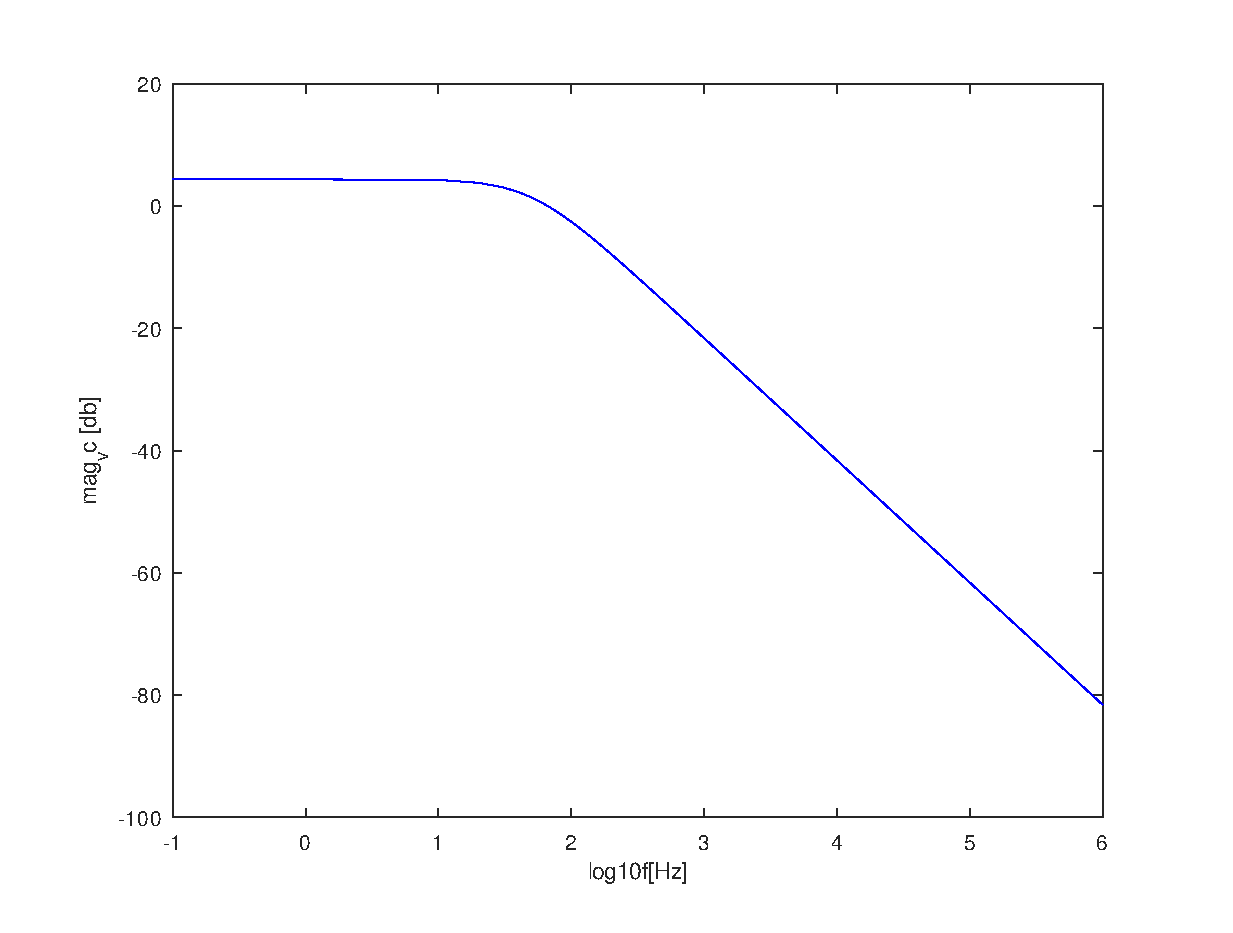
\includegraphics[width=0.49\textwidth]{mag_vc.eps}} 
            \subfigure[]{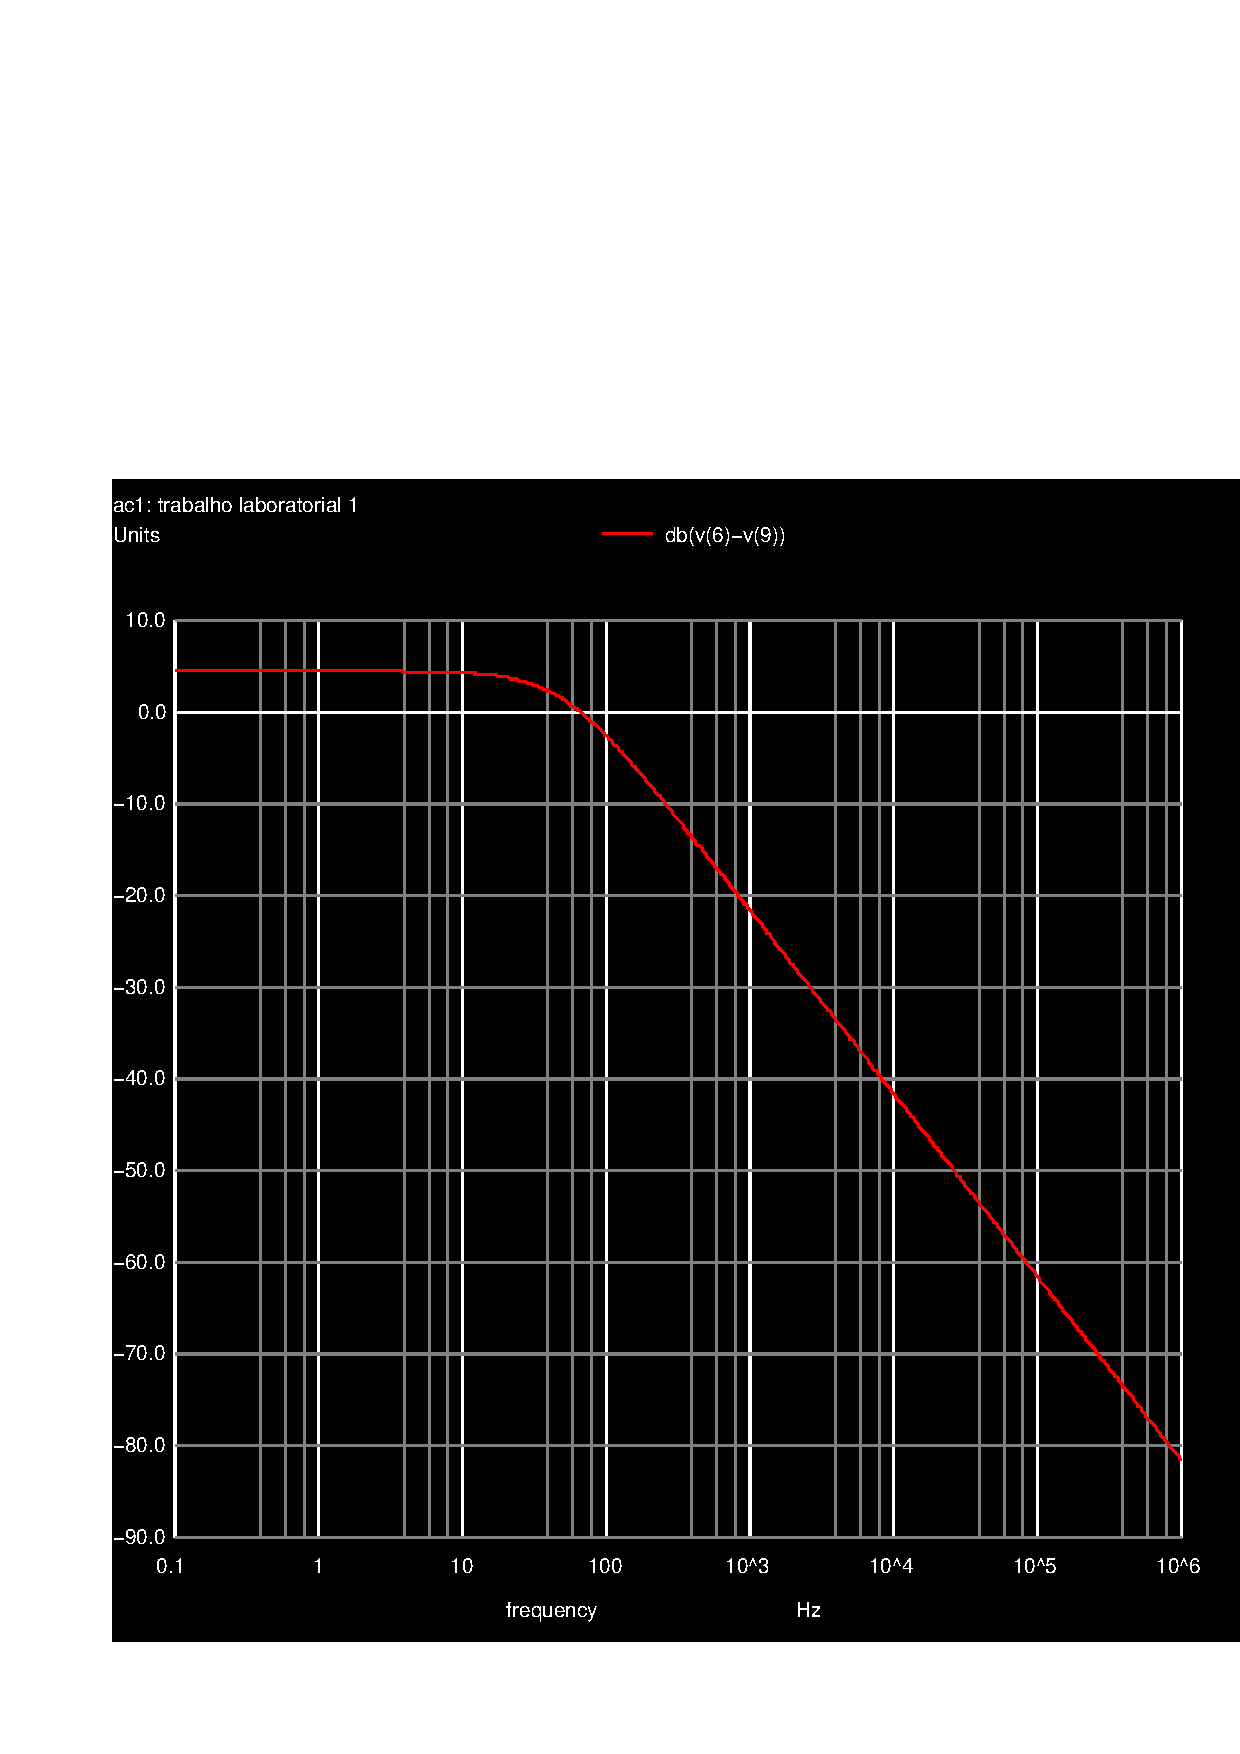
\includegraphics[width=0.42\textwidth]{trans4.pdf}} 
            \caption{(a) Magnitude of Vc in function of frequency using octave (b) Magnitude of Vc in function of frequency using ngspice}
            \label{fig:icere}
\end{figure}
\begin{figure}[h!]
            \centering
            \subfigure[]{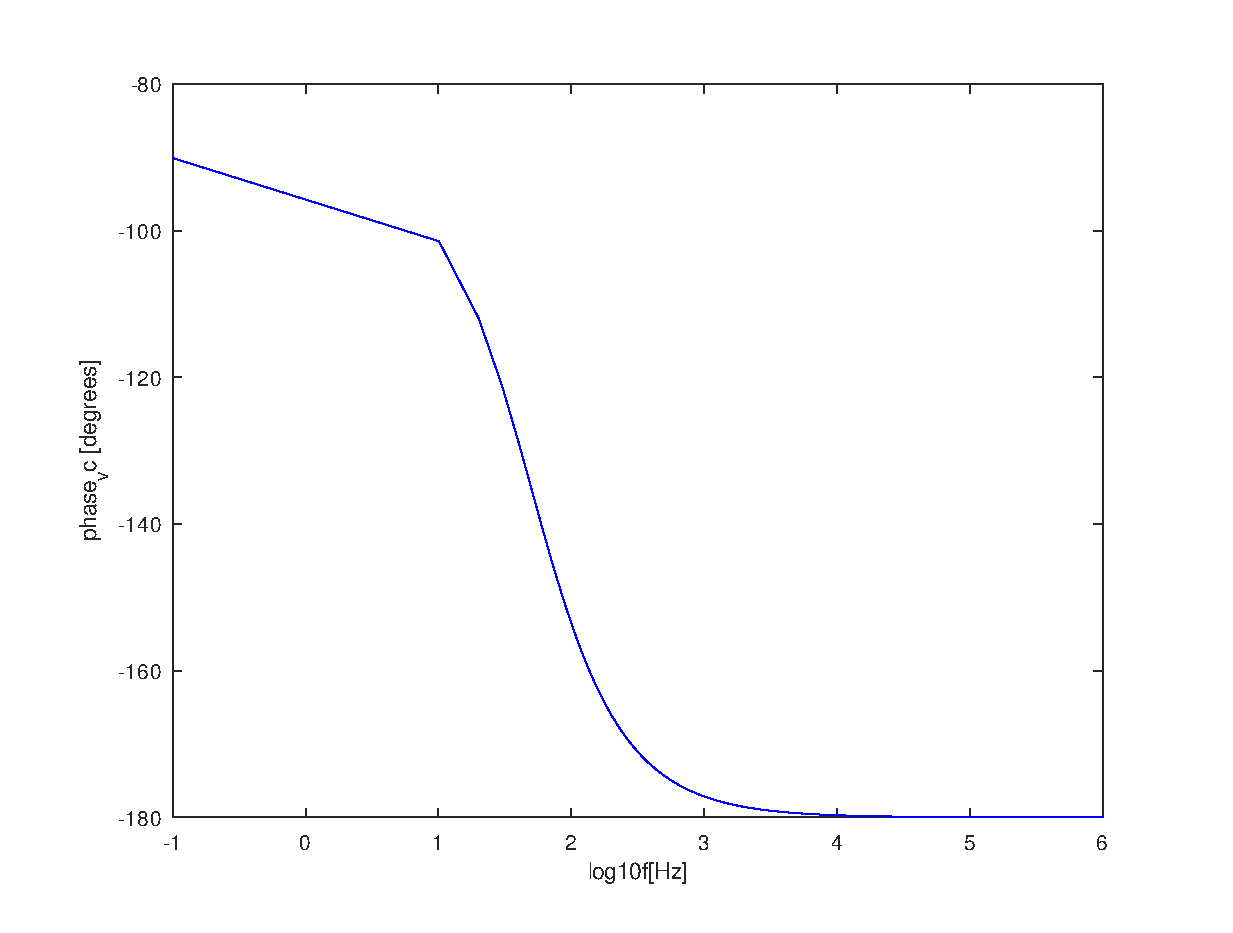
\includegraphics[width=0.49\textwidth]{phase_vc.eps}} 
            \subfigure[]{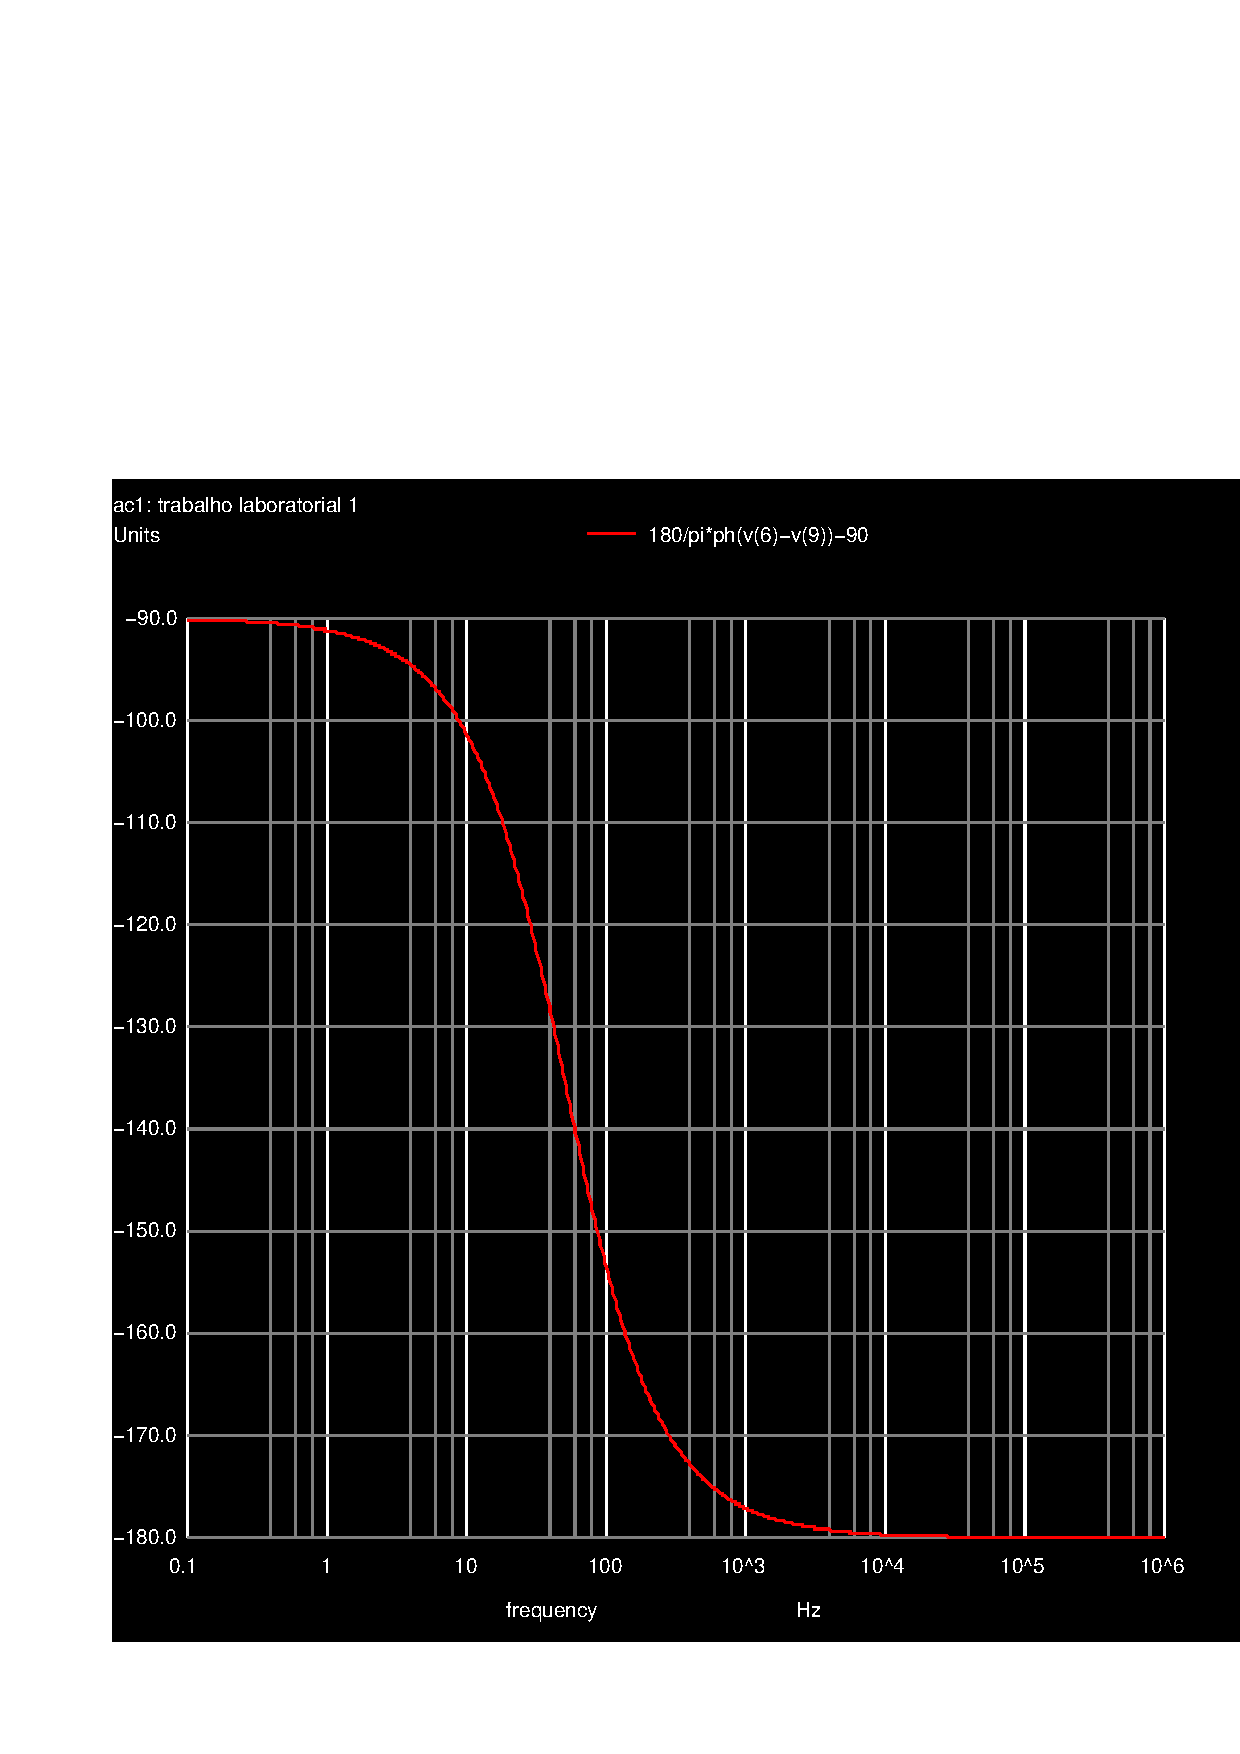
\includegraphics[width=0.42\textwidth]{trans5.pdf}} 
            \caption{(a) Phase of Vc in function of frequency using octave (b) Phase of Vc in function of frequency using ngspice}
            \label{fig:iceer}
\end{figure}

Using octave and ngspice we obtain very similar graphics for phase and magnitude of phasor Vc. Although, they have a few differences in the beginning of the graphic because we have a logaritmic scale
so in the beginning we have much less points that we have in the end.

\newpage

\begin{figure}[h!]
            \centering
            \subfigure[]{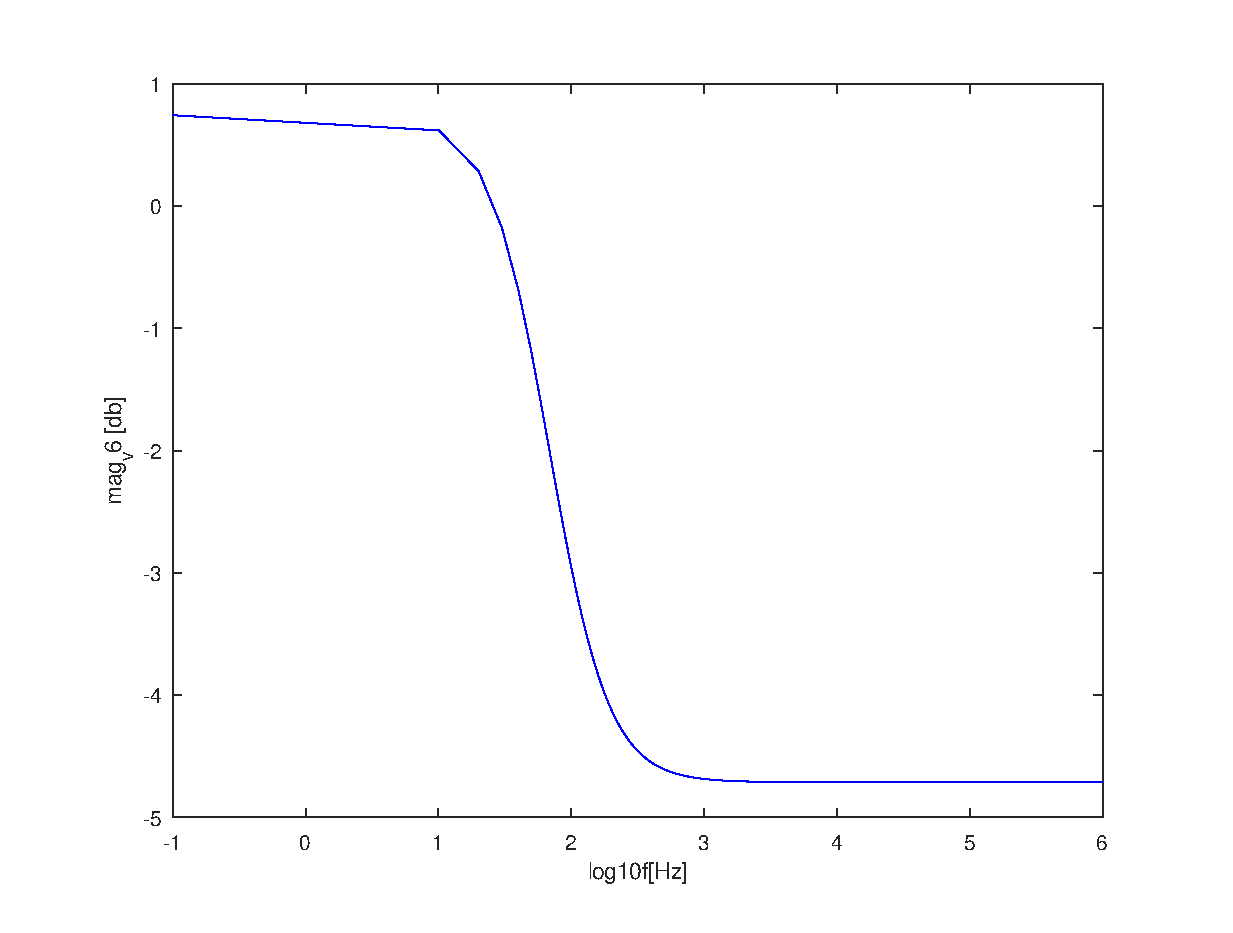
\includegraphics[width=0.49\textwidth]{mag_v6.eps}} 
            \subfigure[]{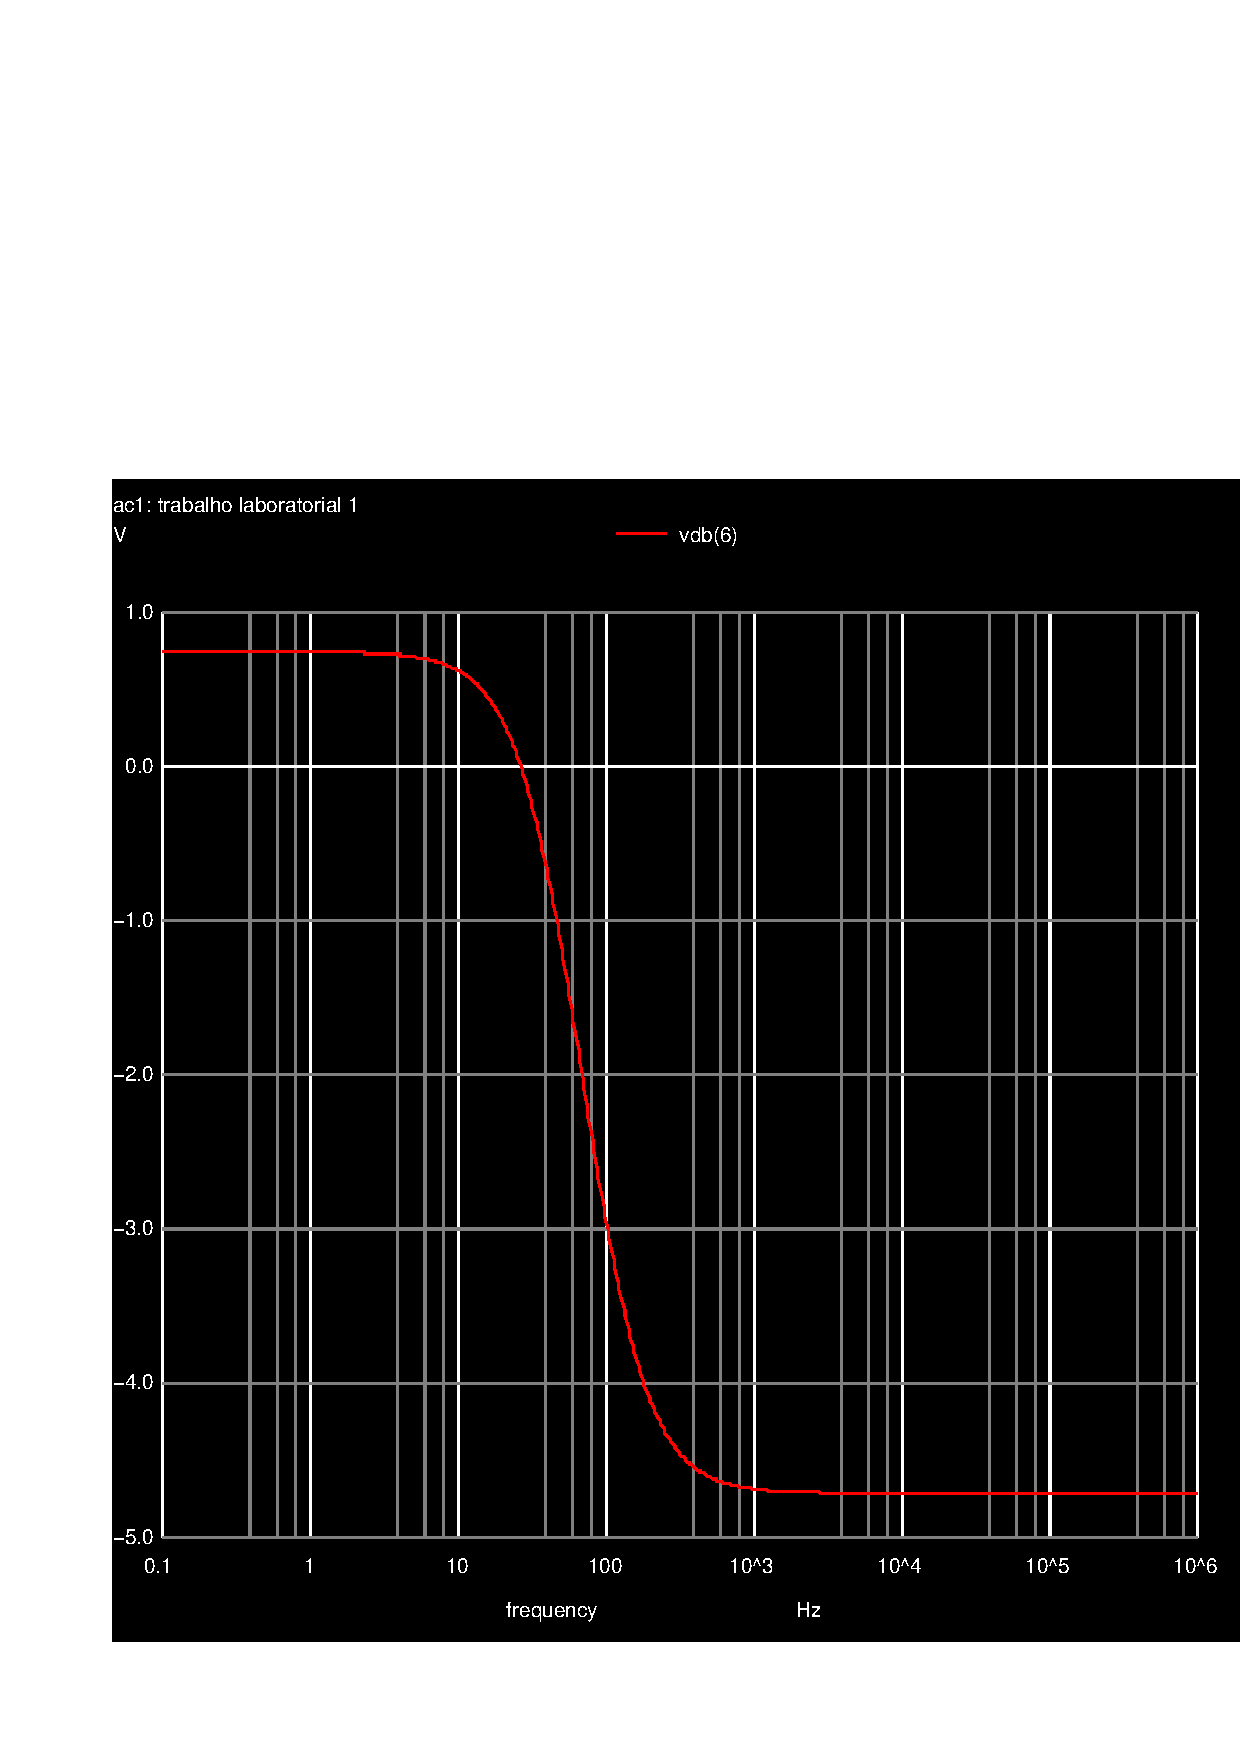
\includegraphics[width=0.42\textwidth]{trans8.pdf}} 
            \caption{(a) Magnitude of V6 in function of frequency using octave (b) Magnitude of V6 in function of frequency using ngspice}
            \label{fig:icase}
\end{figure}
\begin{figure}[h!]
            \centering
            \subfigure[]{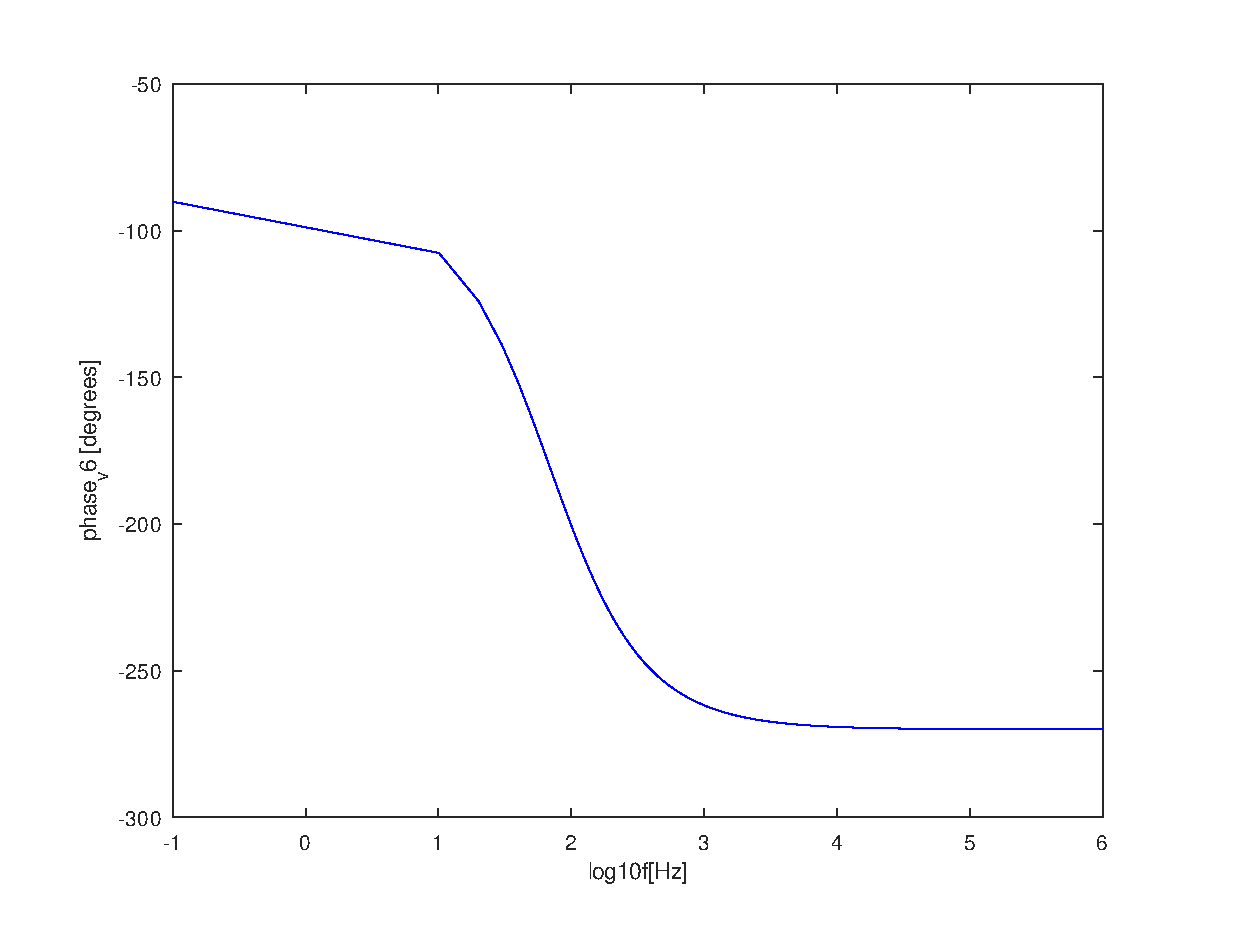
\includegraphics[width=0.49\textwidth]{phase_v6.eps}} 
            \subfigure[]{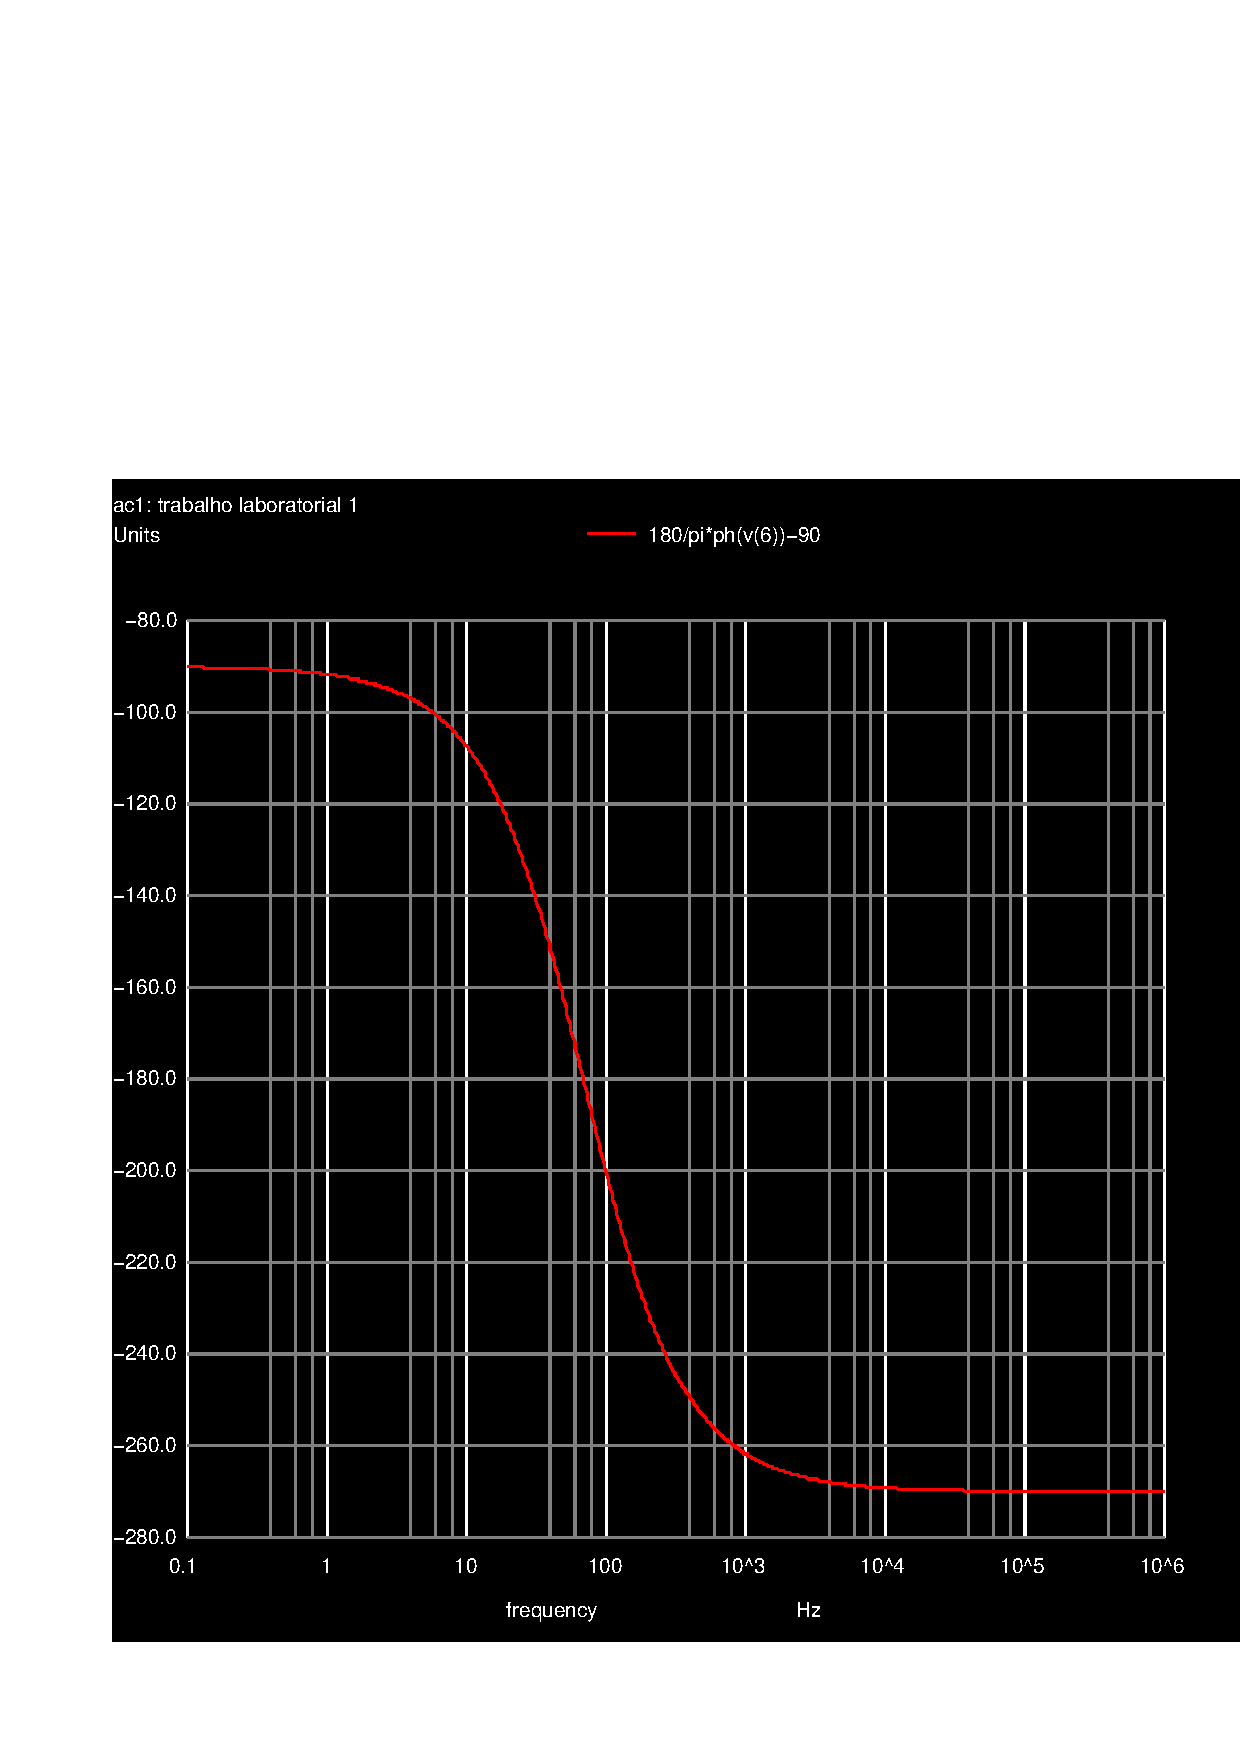
\includegraphics[width=0.42\textwidth]{trans9.pdf}} 
            \caption{(a) Phase of V6 in function of frequency using octave (b) Phase of V6 in function of frequency using ngspcice}
            \label{fig:icere}
\end{figure}

%Using octave and ngspice we obtain very similar graphics for phase and magnitude of phasor V6. Although, they have a few differences in the beginning of the graphic because we have a logaritmic scale
%so in the beginning we have much less points that we have in the end.

\newpage

\begin{figure}[h!]
            \centering
            \subfigure[]{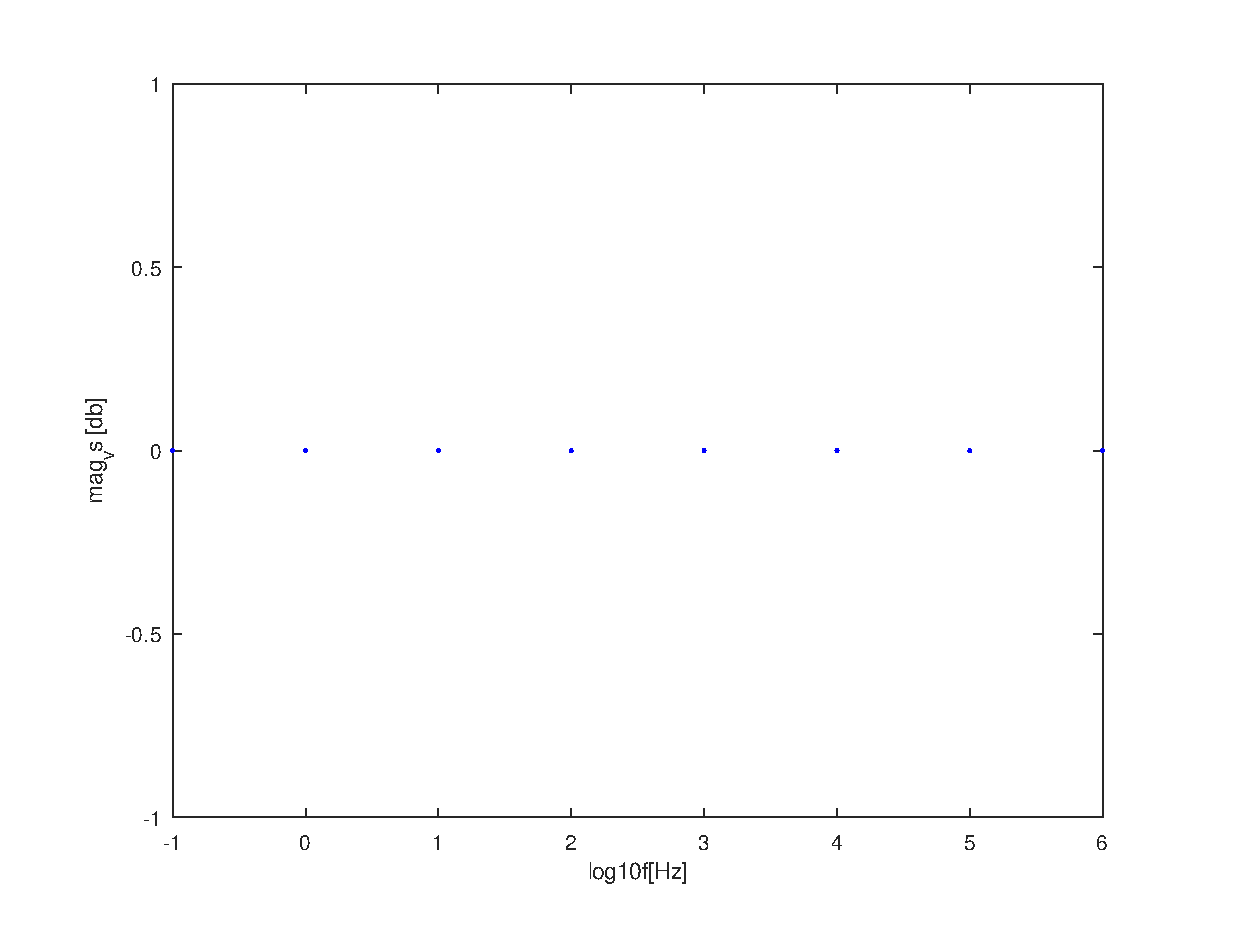
\includegraphics[width=0.49\textwidth]{mag_vs.eps}} 
            \subfigure[]{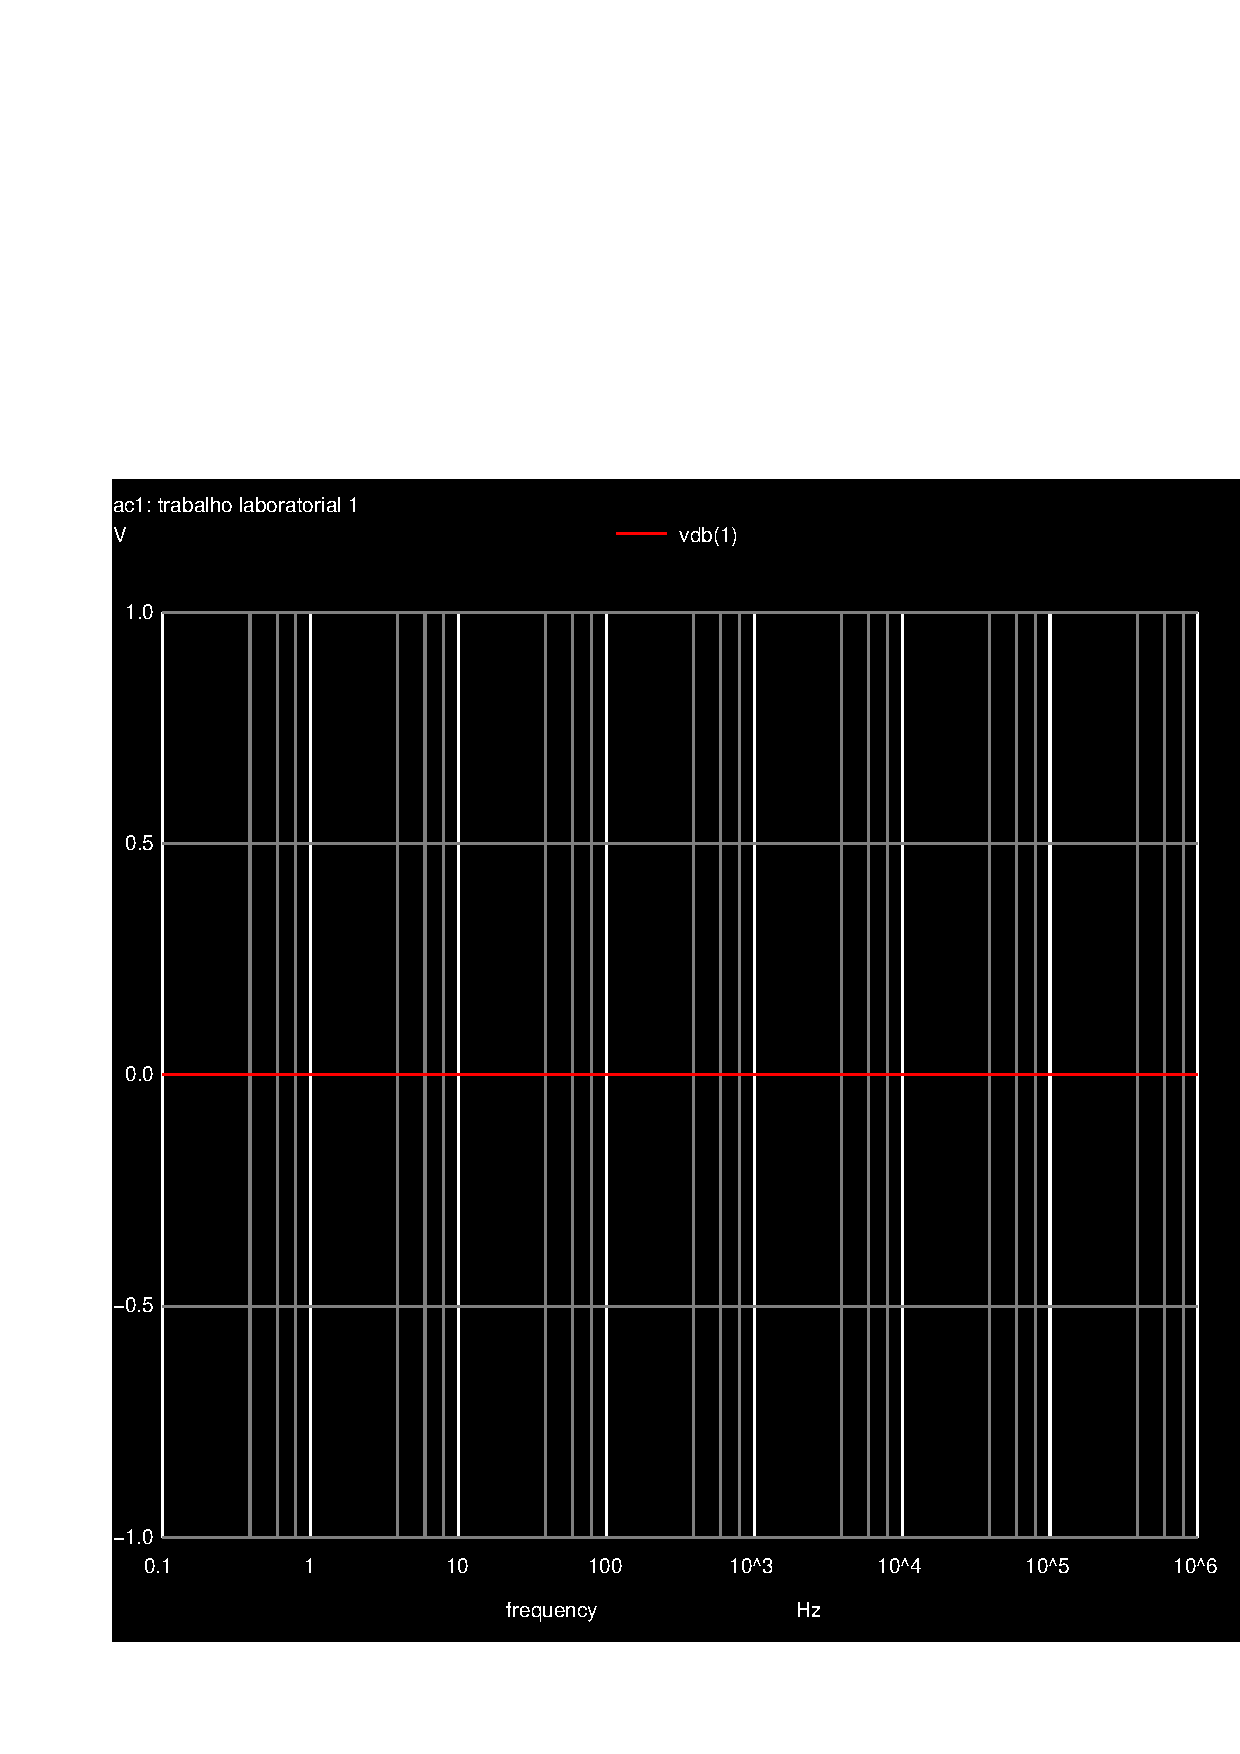
\includegraphics[width=0.42\textwidth]{trans6.pdf}} 
            \caption{(a) Magnitude of Vs in function of frequency using octave (b) Magnitude of Vs in function of frequency using ngspice}
            \label{fig:icefe}
\end{figure}
\begin{figure}[h!]
            \centering
            \subfigure[]{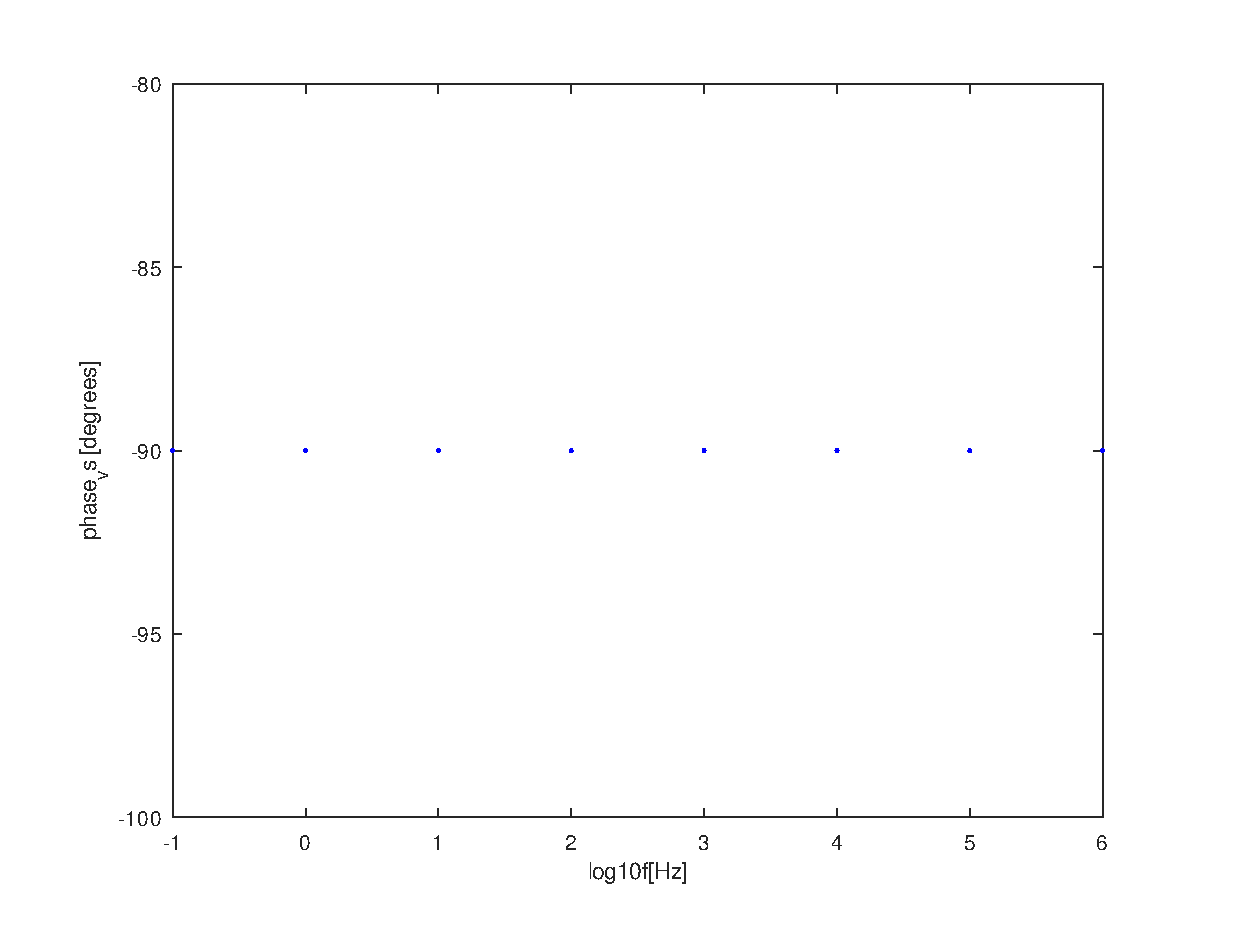
\includegraphics[width=0.49\textwidth]{phase_vs.eps}} 
            \subfigure[]{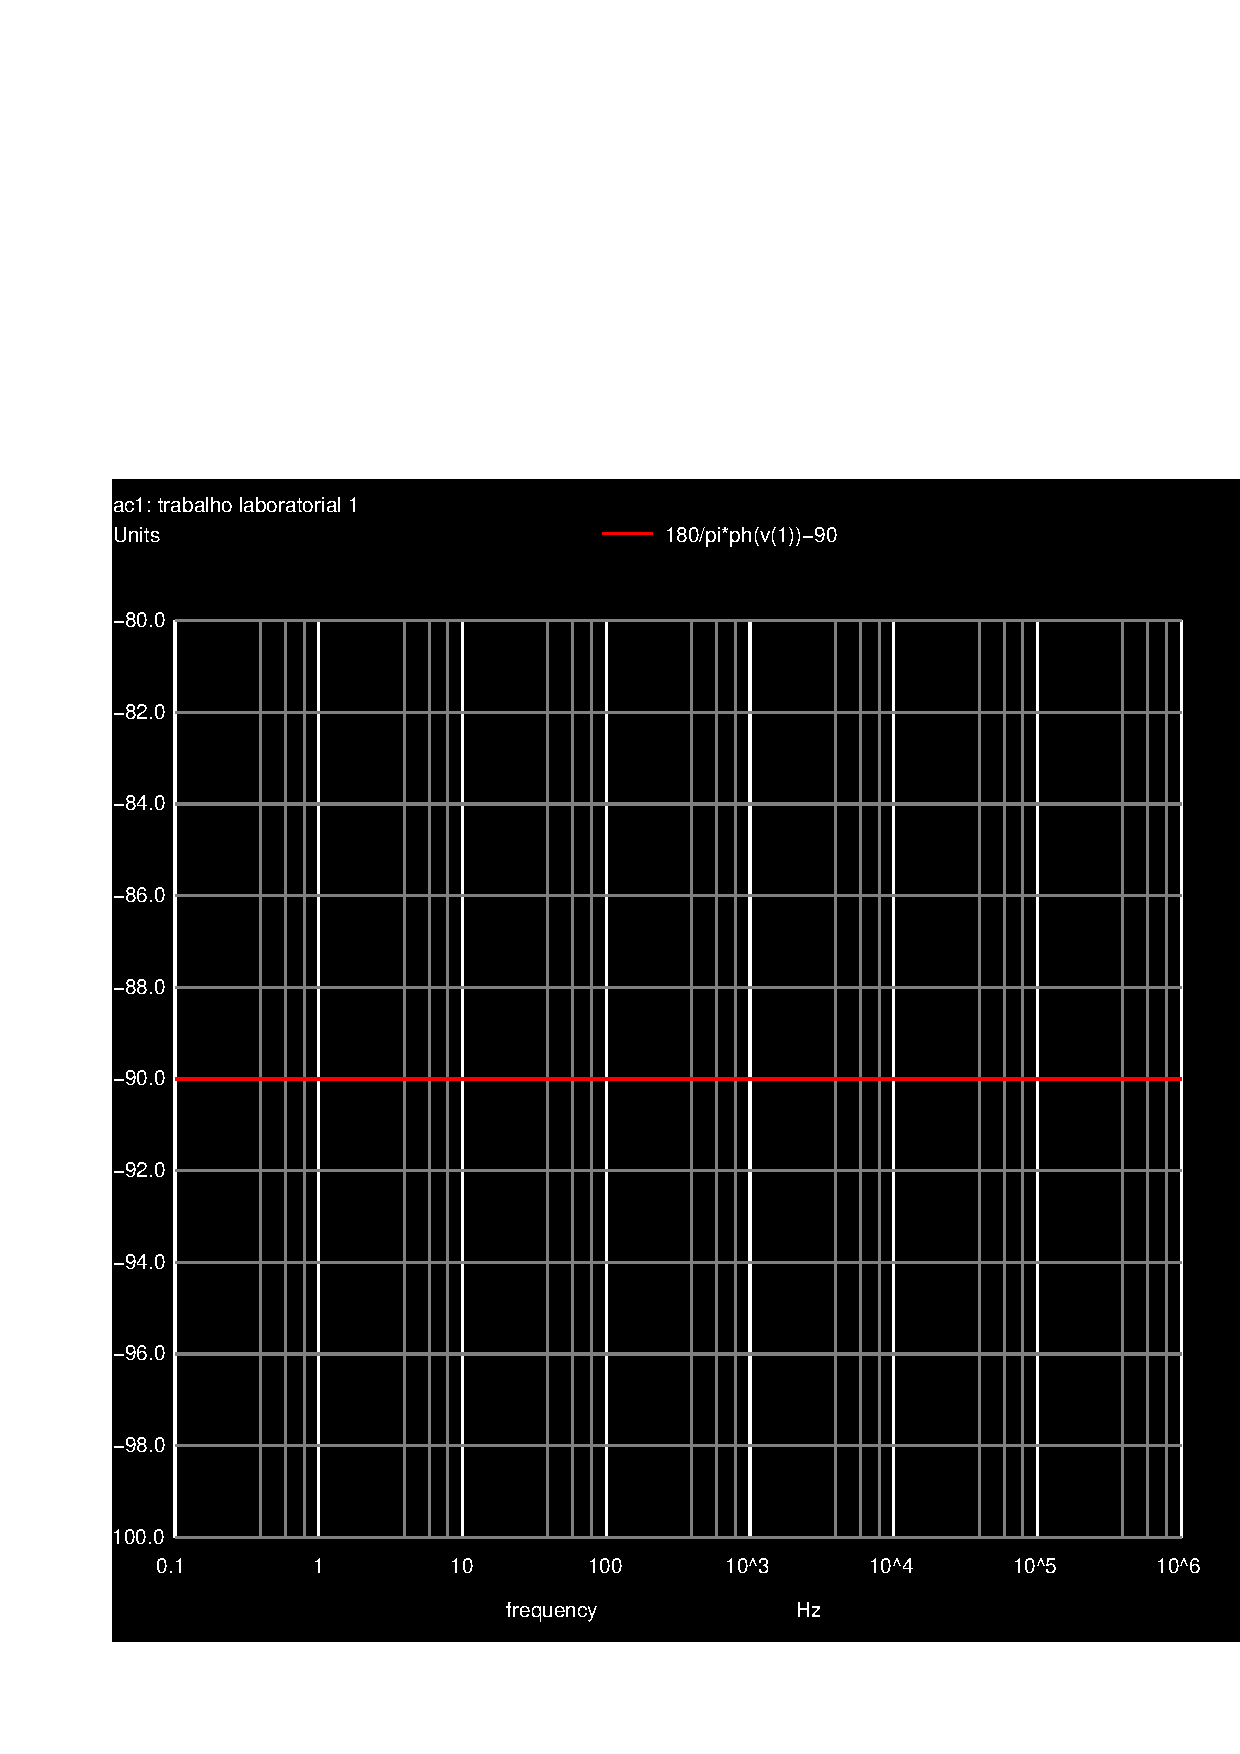
\includegraphics[width=0.42\textwidth]{trans7.pdf}} 
            \caption{(a) Phase of Vs in function of frequency using octave (b) Phase of Vs in function of frequency using ngspice}
            \label{fig:icrgce}
\end{figure}


%Using octave and ngspice we obtain very similar graphics for phase and magnitude of phasor Vs. Although, they have a few differences in the beginning of the graphic because we have a logaritmic scale
%so in the beginning we have much less points that we have in the end.
\newpage
To compare $V_c$ and $V_s$, we can use the following equation, because this represents the RC equivalent transfer function equation.
$$\frac{V_c}{V_s}=\frac{1}{1+j*w*Req*C}$$
Analysing the equation we could understand the differences between the plots of magnitude and phase of $V_c$ and $V_s$.
The magnitude and phase of $V_s$ don't change with the frequency.
To low frequencys, we can see that w is almost zero, so the phase difference is almost none $ph(V_C) = atan(w*Req*C)$ and the magnitude is almost the same.
To high frequencys, we can see that w is tending to infinite, so the phase difference is close to $\frac{\pi}{2}$ and the magnitude of $V_c$ is close to 0. 

To compare $V_c$ and $V_s$ with $V_6$, we must remember that $V_c = V_6-V_8$. If we understand that $V_8$ don't change with frequency, so we know that the graphs of
 $V_c$ will have the same form of the graphics of $V_6$ despite some vertical displacements. And knowing the differences between $V_c$ - $V_s$ and $V_c$ - $V_6$
the differences between $V_s$ - $V_6$ will be direct.



